%!TEX root = ../main.tex

\section{Model Development} % (fold)
\label{sec:model_development}

In order to properly control the double pendulum it is necessary to develop a model of the system.
Throughout this section the model will be developed iteratively.
Initially including only the simple double pendulum, eventually including both friction and the cart.

\subsection{Simple Double Pendulum} % (fold)
\label{sub:simple_double_pendulum}
An illustration of the system can be seen in figure \ref{fig:doublependulum}.
As can be seen, the pendulums have masses $m_1$, $m_2$, suspended using rods of lengths $l_1$, $l_2$.
The rods are assumed to be massless.
The angles of the pendulums $\theta_1$, $\theta_2$, are measured as the offset from the stable position.
For convenience the two pendulums will be referred to as $p_1$ and $p_2$ where $p_2$ is suspended from $p_1$.

\begin{figure}
	\centering
	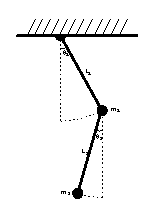
\includegraphics[width=.5\linewidth]{graphics/double_pendulum.eps}
	\caption{Illustration of the simple double pendulum.}
	\label{fig:doublependulum}
\end{figure}

Equations should be developed such that, given an initial state, the position and subsequent movement can be derived from them.
This can be achieved using the Euler-Lagrange differential equations.
These will be found for this system throughout the remainder of this section.
Firstly, the position of the pendulums as a function of the angle must be determined.
The pendulums are placed in the x-y plane with the origin placed at the point of suspension of $p_1$.
When the pendulums are in the stable position, $\theta_1=\theta_2=0$, they are aligned with the y-axis.
The x-axis is positive to the right of the stable position.
The coordinates of $p_1=(x_1,y_1)$ and $p_2=(x_2,y_2)$ are as follows:
\begin{align}
	x_1 &= l_1\sin{\theta_1}\\
	y_1 &= -l_1\cos{\theta_1}\\
	x_2 &= l_1\sin{\theta_1} + l_2\sin{\theta_2}\\
	y_2 &= -l_1\cos{\theta_1} - l_2\cos{\theta_2}
\end{align}
While the derivatives are not used until later, they are presented here for clarity:
\begin{align}
	\dot{x}_1 &= l_1\cos{\theta}_1\dot{\theta}_1\\
	\dot{y}_1 &= l_1\sin{\theta}_1\dot{\theta}_1\\
	\dot{x}_2 &= l_1\cos{\theta}_1\dot{\theta}_1 + l_2\cos{\theta_2}\dot{\theta}_2\\
	\dot{y}_2 &= l_1\sin{\theta}_1\dot{\theta}_1 + l_2\sin{\theta_2}\dot{\theta}_2
\end{align}
In order to calculate the Euler-Lagrange diff. eq. it is necessary to first determine the lagrangian, $\mathcal{l}$:
\begin{equation}
	\mathcal{L}=E_k-E_p
\end{equation}
Where $E_k$ is the kinetic energy of the system and $E_p$, the potential energy.
The derivation of $E_p$:
\begin{align}
	E_p &= m_1 g y_1 + m_2 g y_2\\
		&= -m_1 g l_1 \cos{\theta_1} - m_2 g l_1 \cos{\theta_1} - m_2 g l_2 \cos{\theta_2}\\
		&= -(m_1+m_2)l_1g \cos{\theta_1}-m_2 g l_2 \cos{\theta_2}
		\label{eq:ep}
\end{align}
The derivation of $E_k$:
\begin{equation}
	\label{eq:ek}
	E_k = \frac{1}{2}m_1v_1^2+\frac{1}{2}m_2v_2^2
\end{equation}
As movement is present along both axes, the total velocity of either pendulum can be found as the derivative of the position and Pythagoras:
\begin{align}
	v_1^2 &= \dot{x}_1^2+\dot{y}_1^2\\
		&= l_1^2\dot{\theta}_1^2\cos{\theta}_1^2+l_1^2\dot{\theta}_1^2\sin{\theta_1}^2\\
		&= (\cos{\theta_1}^2+\sin(\theta_1)^2)l_1^2\dot{\theta}_1
\end{align}
Using the Pythagorean identity:
\begin{equation}
	\label{eq:v1}
	v_1^2 = l_1^2\dot{\theta}_1^2
\end{equation}
Similarly:
\begin{align}
	v_2^2 &= \dot{x}_2^2+\dot{y}_2^2\\
	&= (l_1\cos{\theta}_1\dot{\theta}_1 + l_2\cos{\theta_2}\dot{\theta}_2)^2+(l_1\sin{\theta}_1\dot{\theta}_1 + l_2\sin{\theta_2}\dot{\theta}_2)^2\\
	\begin{split}
		&= l_1^2\dot\theta_1^2\cos{\theta_1}^2+l_2^2\dot\theta_2^2\cos{\theta_2}^2+2l_1l_2\dot\theta_1\dot\theta_2\cos{\theta_1}\cos{\theta_2}\\
		&\qquad +l_1^2\dot\theta_1^2\sin{\theta_1}^2+l_2^2\dot\theta_2\sin{\theta_2}+2l_1l_2\dot\theta_1\dot\theta_2\sin{\theta_1}\sin{\theta_2}
	\end{split}
\end{align}
Isolating cosine and sine from the terms pairwise, 1 and 4, 2 and 5, 3 and 6, yields:
\begin{align}
	\begin{split}
		v_2^2&=(\cos{\theta_1}^2+\sin{\theta_1}^2)l_1^2\dot\theta_1^2+(\cos{\theta_2}^2+\sin{\theta_2}^2)l_2^2\dot\theta_2^2\\
	&\qquad+(\cos{\theta_1}\cos{\theta_2}+\sin{\theta_1}\sin{\theta_2})2l_1l_2\dot\theta_1\dot\theta_2
	\end{split}
\end{align}
By applying the trigonimetric identities:
\begin{align}
	1&=\sin{\alpha^2}+\cos{\beta^2}\\
	\cos{(\alpha\pm\beta)}&=\cos\alpha\cos\beta\pm\sin\alpha\sin\beta
\end{align}
The result is found:
\begin{equation}
	\label{eq:v2}
	v_2^2=l_1^2\dot\theta_1^2+l_2^2\dot\theta_2^2+2l_1l_2\dot\theta_1^2\dot\theta_2^2\cos{(\theta_1-\theta_2)}
\end{equation}
Using equations \ref{eq:ep}, \ref{eq:ek}, \ref{eq:v1} and \ref{eq:v2} the lagrangian can be constructed:
\begin{align}
	\begin{split}
		\mathcal{L}&=\frac{1}{2}m_1l_1\dot\theta_1^2+\frac{1}{2}m_2\left(l_1^2\dot\theta_1^2+l_2^2\dot\theta_2^2+2l_1l_2\dot\theta_1^2\dot\theta_2^2\cos{(\theta_1-\theta_2)}\right)\\
		&\qquad+(m_1+m_2)l_1g\cos{\theta_1}+m_2l_2g\cos{\theta_2}
	\end{split}\\
	\begin{split}
		&=\frac{m_1l_1^2\dot\theta_1^2}{2}+\frac{m_2l_1^2\dot\theta_1^2}{2}+\frac{m_2l_2^2\dot\theta_2^2}{2}+l_1l_2\dot\theta_1^2\dot\theta_2^2\cos{(\theta_1-\theta_2)}\\
		&\qquad+(m_1+m_2)l_1g\cos{\theta_1}+m_2l_2g\cos{\theta_2}
	\end{split}
\end{align}
Which simplifies to:
\begin{equation}
	\label{eq:lagrangian}
	\mathcal{L}=\frac{(m_1+m_2)l_1^2\dot\theta_1^2}{2}+\frac{m_2l_2^2\dot\theta_2}{2}+(m_1+m_2)l_1g\cos{\theta_1}+m_2l_2g\cos{\theta_2}\\
\end{equation}
The Euler-Lagrange diff. eq. are defined as:
\begin{equation}
	\frac{d}{dt}\left(\frac{\partial \mathcal{L}}{\partial \dot\theta}\right)-\frac{\partial \mathcal{L}}{\partial \theta} = 0
\end{equation}
The three terms $\frac{\partial \mathcal{L}}{\partial \dot\theta}$,$\frac{d}{dt}\left(\frac{\partial \mathcal{L}}{\partial \dot\theta}\right)$ and $\frac{\partial l}{\partial \theta}$ are calculated next for each of the pendulums. For $p_1$:
\begin{align}
	\frac{\partial \mathcal{L}}{\partial \dot\theta_1}&=(m_1+m_2)l_1^2\dot\theta_1+m_2l_1l_2\dot\theta_2\cos{(\theta_1-\theta_2)}\\
	\begin{split}
		\frac{d}{dt}\left(\frac{\partial \mathcal{L}}{\partial \dot\theta_1}\right)&=(m_1+m_2)l_1^2\ddot\theta_1+m_2l_1l_2\ddot\theta_2\cos{(\theta_1-\theta_2)}\\
		&\qquad-m_2l_1l_2\dot\theta_2\sin{(\theta_1-\theta_2)(\dot\theta_1-\dot\theta_2)}
	\end{split}\\
	\frac{\partial \mathcal{L}}{\partial \theta_1} &= -m_2l_1l_2\dot\theta_1\dot\theta_2\sin(\theta_1-\theta_2)-(m_1+m_2)l_1g\sin{\theta_1}\\
	\begin{split}
		0&=(m_1+m_2)l_1\ddot\theta_1+m_2l_2\ddot\theta_2\cos{(\theta_1-\theta_2)}\\
		&\qquad+m_2l_2\dot\theta_2^2\sin{(\theta_1-\theta_2)}+(m_1+m_2)g\sin{\theta_1}
	\end{split}
\end{align}
And $p_2$:

\begin{align}
	\frac{\partial \mathcal{L}}{\partial \dot\theta_2}&=m_2l_2^2\dot\theta_2+m_2l_1l_2\dot\theta_1\cos{(\theta_1-\theta_2)}\\
	\begin{split}
		\frac{d}{dt}\left(\frac{\partial \mathcal{L}}{\partial \dot\theta_2}\right)&=m_2l_2^2\ddot\theta_2+m_2l_1l_2\ddot\theta_1\cos{(\theta_1-\theta_2)}\\
		&\qquad -m_2l_1l_2\dot\theta_1\sin{(\theta_1-\theta_2)}(\dot\theta_1-\dot\theta_2)
	\end{split}\\
	\frac{\partial \mathcal{L}}{\partial \theta_2} &=m_2l_1l_2\dot\theta_1\dot\theta_2\sin{(\theta_1-\theta_2)}-m_2l_2g\sin{\theta_2}\\
	\label{eq:part}
	\begin{split}
		0&=m_2l_2\ddot\theta_2+m_2l_1\ddot\theta_1\cos{(\theta_1-\theta_2)}\\
		&\qquad-m_2l_1\dot\theta_1^2\sin{(\theta_1-\theta_2)}+m_2g\sin{\theta_2}
	\end{split}
\end{align}
\thomas{eq. \ref{eq:part} has a minus in front of the first term according to our calculations. Determine why.}
% subsection simple_double_pendulum (end)

% section model_development (end)
